CrowdNote was developed as a classic Web system. To facilitate the sharing of software produced, only technologies that do not require complex infrastructure were adopted. The server was fully developed in NodeJS for easy deployment, the client was developed in HTML 5 to improve compatibility and the persistence layer uses MongoDB as No-SQL database.

The architecture of the CrowdNote is illustrated in Figure~\ref{architecture} in which is possible observe the 3 main components: Server, Database and Clients.

\begin{figure}[h!]
	\centerline{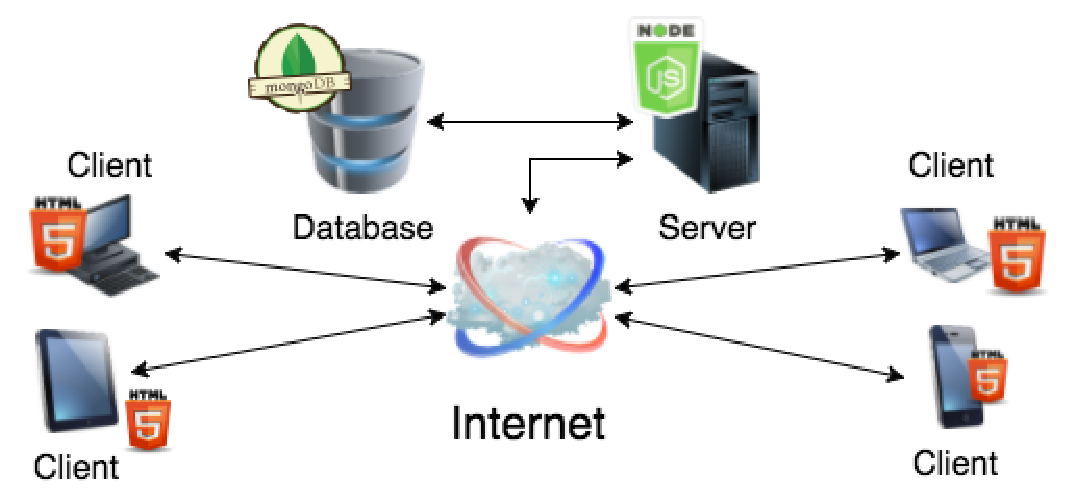
\includegraphics[scale=0.3] {figure/Architecture}}
	\caption{CrowdNote Architecture}
	\label{architecture}
\end{figure}

\subsection{Persistence}
The persistence was addressed using MongoDB, that deliver a very interesting solution to build No-SQL databases with some characteristics that meets the crowdsourcing requirements such as: high write load, high availability in an unreliable environment,  easy scaling and partition, heterogeneous data into the same collection.

In this model, JSON document collections are used instead of tables, and the documents in each collection may have a different structure to store different attributes. This feature allowed the modeling of a very simple database structure, composed of 3 collections of documents, as can be seen in Figure~\ref{persistence}. It was possible because documents in the Input and Output collections can contain different fields according to the task that consumes or generates the entries.

The Video collection stores entries related to the video segments dataset, the Input collection stores the input entries to the tasks, and the Output collection stores the contributions collected from the crowd.

\begin{figure}[h]
	\centerline{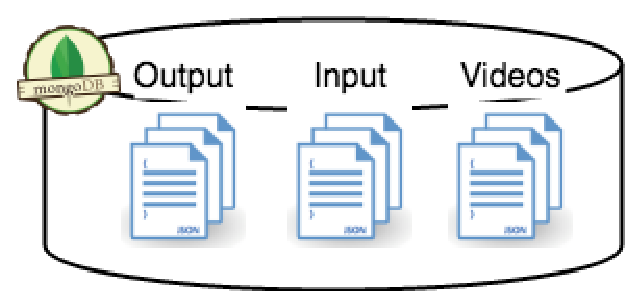
\includegraphics[scale=0.3] {figure/Persistence}}
	\caption{No-SQL Database - JSON Documents Collections}
	\label{persistence}
\end{figure}


\subsection{Workflow}

The internal workflow followed by CrowdNote is ilustrated by Figure~\ref{workflow}. The server system is composed by 3 modules: Collector, Aggregator and Player Provider.

\begin{figure}[h]
	\centerline{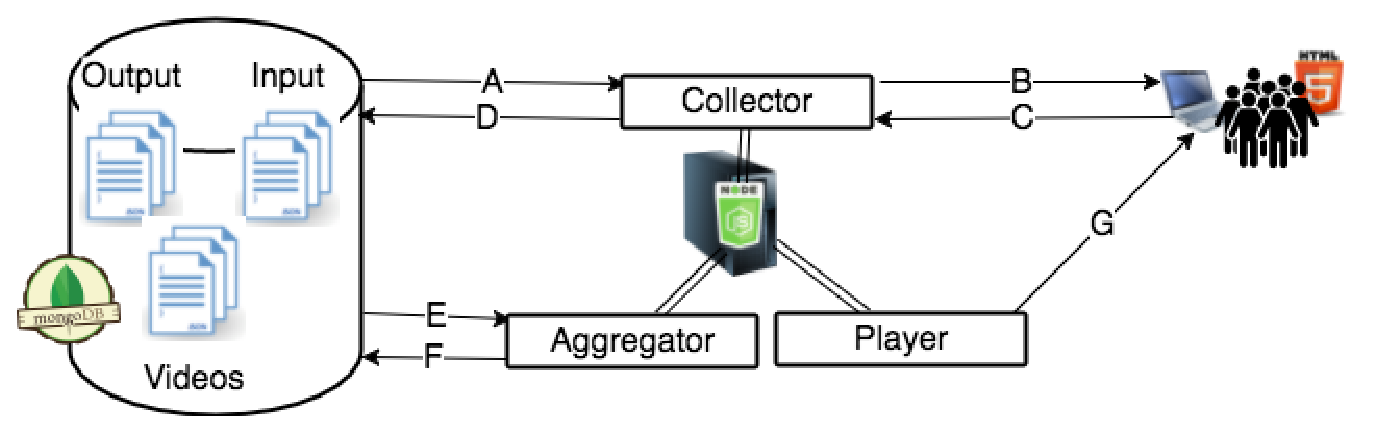
\includegraphics[scale=0.4] {figure/Workflow}}
	\caption{CrowdNote Workflow}
	\label{workflow}
\end{figure}

\textbf{Collector: } For each job request from the client, the Collector receive a register from the Input collection, that defines the annotation to be collected, and the respective media from the video collection (\textbf{A}). These information is used to generate the job view that sends it to a client (\textbf{B}) that renders it. A worker execute the job and this contribution is sent to Collector (\textbf{C}). Finally, the Collector store the contribution into the Output collection (\textbf{D}).

\textbf{Aggregator: } When a task is finished, the Aggregator receive all contributions into the Output collection related with that task (\textbf{E}). Aggregator applies the rules defines for the task to verify and process the contributions, so the result entries are stored into the Input collection (\textbf{F}), and these entries will be the new input to the next task.

\textbf{Player Provider: } When the Aggregator process the contributions for the last task, the result entries are stored into the Input collection as input for the Player Provider. This component sends to client instances the media and meta-data required to play the enriched videos (\textbf{G}).

